\chapter{Training General-Purpose Coding Agents with Constitution Development (\textit{proposed})}
\label{chap:effective-analysis}



\begin{table}[t]
\centering
\small
\resizebox{0.9\columnwidth}{!}{%
\begin{tabular}{l ccc}
\toprule
\multirow{2}{*}{\bf Teacher Model (|Train Size|} &
\multicolumn{3}{c}{\bf SWE-bench Verified (Easy 50)} \\
\cmidrule(lr){2-4}
& Resolved \% & Localized \% & Non-Empty \% \\
\midrule
\sdlrow & \multicolumn{3}{c}{\textit{Base Model: Qwen2.5Coder-7B}} \\
\midrule
\textemdash & \worse 2.0 & 4.0 & 8.0 \\
\midrule
Qwen2.5Coder-32B (399) & \bad 4.0 & 20.0 & 48.0 \\
Qwen2.5Coder-32B + \plusname (399) & \good 8.0 & 46.0 & 68.0 \\
Claude-Sonnet-3.7 (399)   & \better \bf 26.0 & 68.0 & 86.0 \\
\bottomrule
\end{tabular}%
}
\caption{Results on training Qwen2.5Coder-7B on successful trajectories of the exact same 399 function localization instances generated by Qwen2.5Coder-32B and Claude-3.7. 
We evaluate the models on a subset of the SWE-bench Verified issue-solving dataset after training. 
}
\label{ablation:self-vs-claude}
\end{table}


\section{Introduction}

In \autoref{chap:hybrid-gym}, we introduce Hybrid-Gym~\cite{hybrid-gym}, which trains a general-purpose coding agent by deriving a set of training task design principles. 
However, having proper training tasks is not the only condition for effective coding agent training.

In addition to training tasks, both Hybrid-Gym and previous work discover other crucial factors of the training outcome.
Most analyses focus on the standard rejection sampling finetuning setting~\cite{rejection-sampling}, where we apply a teacher model to solve a set of problem instances, select successful trajectories by running evaluation, and train the student model on successful trajectories.
In particular, SWE-Gym~\cite{swegym} and SWE-Smith~\cite{swe-smith} find that training instances with a balanced difficulty distribution improve training results.
RepoST~\cite{repost}, SWE-Smith~\cite{swe-smith}, and Hybrid-Gym~\cite{hybrid-gym} demonstrate that it is beneficial to cover diverse repositories in the training data.
Hybrid-Gym~\cite{hybrid-gym} shows that training on trajectories with more steps improves performance.

One of the discoveries from Hybrid-Gym~\cite {hybrid-gym} is that \textbf{even successful trajectories generated from the same set of instances may have substantially different impact in training}.
As shown in \autoref{ablation:self-vs-claude}, we use Claude-Sonnet-3.7 and Qwen2.5Coder-32B to generate successful trajectories on the exact same set of 399 function localization instances and train Qwen2.5Coder-7B on these successful trajectories, separately.
Surprisingly, the model distilled from Claude-3.7 achieves much better performance than the model distilled from Qwen2.5Coder-32B, in terms of the resolved rate, localization rate, and non-empty rate on SWE-Bench-Verified \cite{swebench}.
After manually examining the training trajectories, we observe the following major differences: Claude's trajectories have more reasonable repo-exploration strategies, more thinking, and more solution verification. This indicates that such ``agent behaviors'' beyond task success substantially affect training outcome.

Most existing works directly use the latest and most powerful model as the teacher model to construct training data~\cite{swegym,R2EGym,swe-smith,swe-play}, including our Hybrid-Gym work~\cite{hybrid-gym}, which typically cost substantially more than weaker but more cost-efficient models. 
For instance, Claude-Sonnet-3.7 costs \$3.00 per million input tokens, while Qwen2.5Coder-32B only costs \$0.03.
With the ultimate goal of conducting feasible, effective, and generalizable coding agent training, \textbf{we aim to develop a task-agnostic and model-agnostic pipeline to improve the quality of training trajectories for general coding agent training tasks}. 
By limiting the usage of strong yet expensive models in our pipeline, we reduce the costs of generating training trajectories while maintaining effectiveness.
Furthermore, by revealing the agent behaviors in training trajectories that are potentially beneficial or harmful for training outcome, we enable future research to determine the quality of training data before running actual training and evaluation.

In this project, given a weak teacher model (e.g., Qwen2.5Coder-32B), we propose \plusname, a trajectory augmentation framework that identifies agent behaviors by comparing to a strong teacher model (e.g., Claude-3.7), augments training trajectories by adding or reducing such behaviors, and finally determines whether they are beneficial or harmful by training a student model again.
In particular, we first generate successful trajectories with a strong teacher model and a weak teacher model on a small set of instances. Then we leverage an LLM to compare each pair of successful trajectories, identify the differences in the strong and weak models' behaviors, and summarize its findings.
% (e.g., strong models have more comprehensive repository exploration strategies)
After obtaining a list of different behaviors, we verify that such differences generally exist by statistical analysis.
% (e.g., by checking the percentage of trajectories that conduct repository exploration by file searching, function searching, and function understanding).
To determine whether each behavior is beneficial or harmful, we inject it or remove it from the weak model's trajectories with three types of methods: adding corresponding constitutions (i.e., a set of rules) in the prompt for rollout, using the strong model to provide concise guidance in rollout, and post-editing the trajectories.
Finally, after verifying that the behavior we study is indeed increased or decreased from the weak teacher model's trajectories, we conduct rollout, training the student model with the updated trajectories, and examine evaluation results.
We iteratively run the above steps until we obtain a list of beneficial and harmful agent behaviors and a set of methods to add or remove such behaviors from training trajectories.

To validate our approach, we apply our pipeline on multiple training tasks, including the SWE-Gym issue-solving dataset~\cite{swegym} and the Hybrid-Gym dataset containing four tasks: function localization, issue localization, dependency search, and function generation~\cite{hybrid-gym}.
To validate the proposed trajectory augmentation methods, we evaluate the finetuned student model on multiple coding agent benchmarks: the SWE-Bench issue-solving benchmark~\cite{swebench}, the SWT-Bench test generation benchmark~\cite{swt-bench}, and the Commit-0 library generation benchmark~\cite{commit0}.
The expected experimental results are two-fold: 
for every potential beneficial or harmful trajectory behavior we find, we expect to see that (1) we successfully increase or decrease such behaviors with our pipeline, and (2) increasing or decreasing such behaviors in the training data improves the training of student models.






\section{Proposed Methodology: the \plusname Framework}
As shown in \autoref{fig:plus:framework}, we propose a framework to identify the beneficial and harmful agent behaviors and add/remove them in training trajectories under the rejection sampling finetuning setting (\S\ref{plus:sec:preliminary}).
Given a weak teacher model (e.g., Qwen2.5Coder-32B) and a reference strong model (e.g., Claude-3.7), we first identify the differences between their behaviors in successful trajectories (\S\ref{plus:sec:discovery}). Then we add or remove such behaviors from the weak teacher model's training trajectories by constitution development, collaboration with the strong model, or trajectory post-editing (\S\ref{plus:sec:augmentation}).
Finally, we determine whether such behaviors are beneficial or harmful by training a student model on the updated trajectories (\S\ref{plus:sec:verification}).
The above steps can be iteratively adopted.




\subsection{Preliminary: Rejection Sampling Finetuning}
\label{plus:sec:preliminary}
Following previous work~\cite{swegym,R2EGym,swe-smith,swe-play,hybrid-gym}, we focus on the rejection sampling finetuning setting~\cite{rejection-sampling}:
To construct the training set, we apply a teacher model to solve a set of problem instances, run evaluation, and collect successful trajectories. 
Then we train a student model on the successful trajectories by supervised finetuning (SFT).
As shown in \autoref{chap:hybrid-gym}, the training tasks do not need to be the same as the downstream tasks in evaluation.




\subsection{Agent Behavior Discovery}
Our analysis in \autoref{ablation:self-vs-claude} shows that agent behaviors beyond task success substantially affect training performance. 
The first question to ask is: \textbf{what are the different behaviors in strong and weak teacher models' trajectories?}
To answer this question, we first adopt an LLM (e.g., o3-mini~\cite{o3_mini}) to identify a list of potential differences between the trajectories generated by the strong teacher model and the weak teacher model.
Then we manually design statistical analyses to verify that these differences exist.

\label{plus:sec:discovery}
\start{LLM-based Comparison}
As shown in \autoref{fig:plus:framework}, we start by applying the strong and weak teacher models on the same set of training instances and collect the instances where both of them generate a successful trajectory.
To compare their behaviors when resolving the same task, we apply an LLM to conduct pairwise comparisons and identify the differences in each pair of trajectories, in terms of both the high-level problem-solving strategy and the concrete actions.
Finally, after gathering the differences on a small set of trajectory pairs (we use 30 pairs in our experiments), we apply an LLM again to summarize the pattern of different agent behaviors.

An example of differences in concrete actions is that Claude-3.7 calls the ``think'' action significantly more often than Qwen2.5Coder-32B.
As for high-level strategies, we observe that Claude-3.7~\cite{claude37} adopts different repo-exploration strategies from Qwen2.5Coder-32B~\cite{qwen25coder}. 
Claude-3.7 typically follows the steps of locating relevant Python files by several keywords, locating the concrete functions or classes inside those files by another round of keyword searching, understanding the functionality and usage of the located functions, and finally searching for potential test files.
In comparison, after searching for relevant files with keywords, Qwen2.5Coder-32B~\cite{qwen25coder} directly reads the whole file to locate relevant functions. It never tries to understand the functionality and usage of the functions and never searches for test files.

\start{Verification with Statistical Analysis}
Although LLMs can generate references in its outputs and can even write code to support its findings, the results are still not trustworthy.
As a result, we manually design statistical analyses to determine that the differences in agent behaviors truly exist.

We provide an example in \autoref{fig:plus:framework}, where we break down repo-exploration strategies into quantitative terms.
For instance, we check whether the agent locates functions by keyword searching by matching the following Regular Expressions (RE) patterns: \textit{grep -n ``def \$FUNC'' \$FILE}, \textit{grep -n ``class \$CLASS'' \$FILE}, and \textit{grep -n ``\$KEYWORD'' \$FILE}.


\begin{figure}[t]
\centering
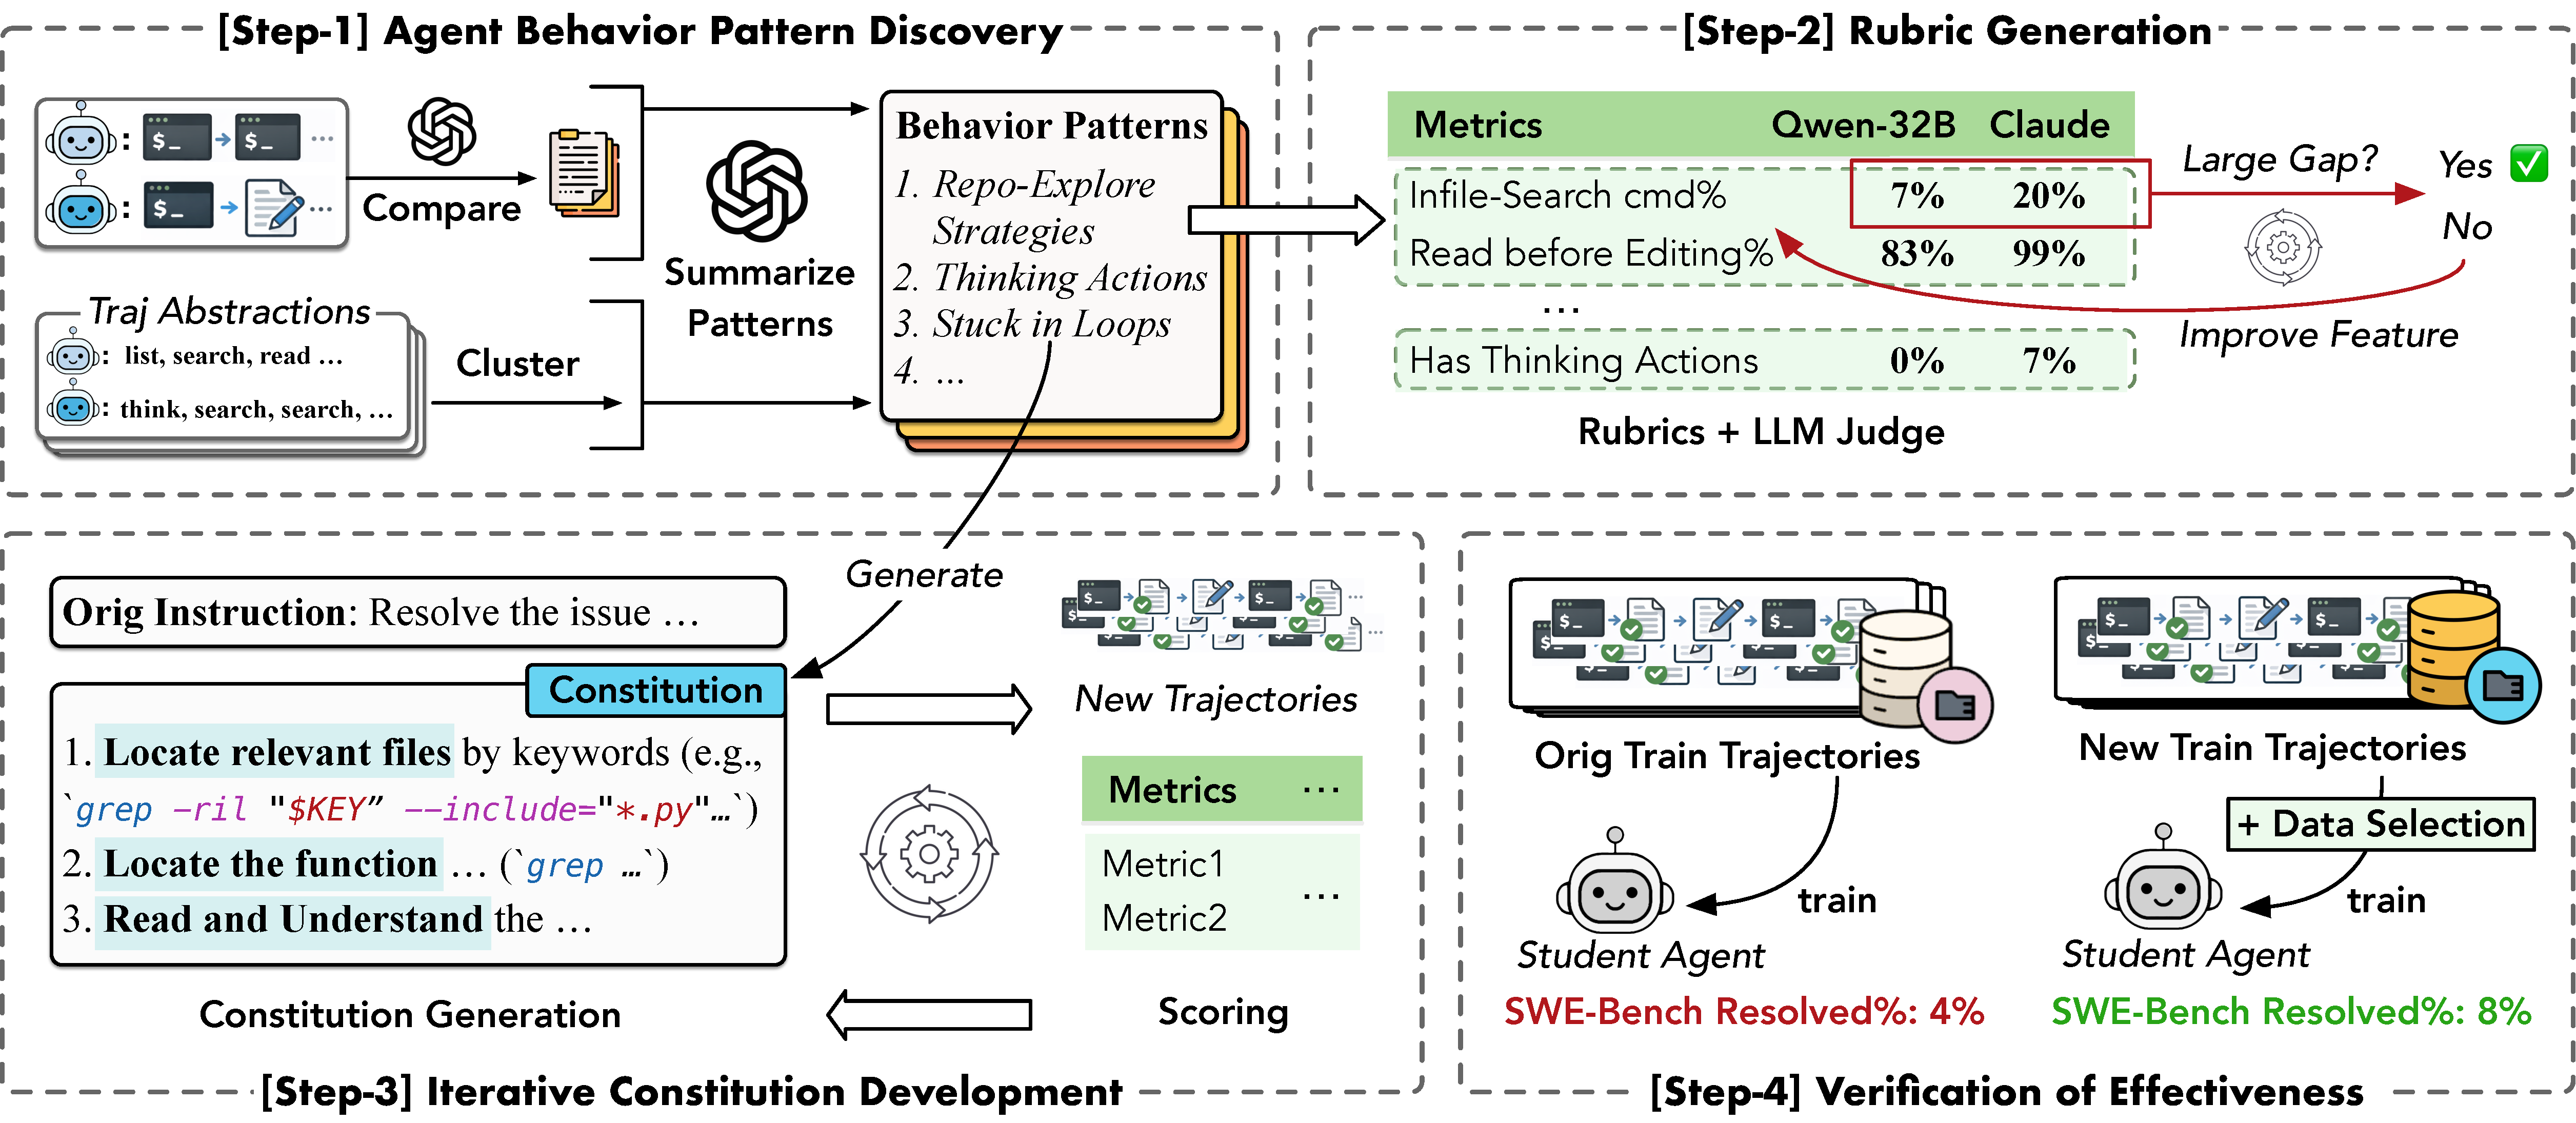
\includegraphics[width=\textwidth]{plus_figs/hybridplus.pdf}
\caption{The \plusname framework. 
(\textit{Upper-Left}) We first discover the different behaviors in the strong and weak teacher models' successful trajectories. 
(\textit{Lower-Left}) Then we augment the weak model's trajectories by injecting the strong model's behaviors.
(\textit{Right}) Finally, after verifying that the desired behaviors are indeed imitated by the weak teacher model, we train a student model on the augmented training trajectories and compare the results with the original training set.
Finally, we go back to Step-1 and continue exploring the differences between the augmented weak teacher model's trajectories from the strong model's trajectories.
}
\label{fig:plus:framework}
\end{figure}




\subsection{Trajectory Augmentation}
\label{plus:sec:augmentation}

While \S\ref{plus:sec:discovery} finds a list of different behaviors in the strong and weak teacher models' trajectories, we do not know yet whether the behaviors affect training performances or whether the behaviors can be easily imitated.
As a result, \textbf{we imitate the strong model's behaviors in the weak model's trajectories with three proposed approaches}. We call this step ``trajectory augmentation''.
The approaches we propose include: writing targeted constitutions in the prompt when generating training trajectories, collaborating with the strong model, and post-editing the trajectories. 

\start{Approach 1: Constitution Development}
The most straightforward method is to improve the prompt of generating training trajectories by adding a list of rules, which are called ``constitutions'' in previous research~\cite{constitutional-ai}.
Here we adopt Constitutional AI's method~\cite{constitutional-ai} that writes the constitution, generates a few examples, uses an LLM to judge whether the constitutions are well satisfied, and refines the prompts, if needed.

\autoref{fig:plus:framework} shows an example of the constitutions we develop. 
The original rollout prompt is concise about repo-exploration: ``explore the codebase to find functions that match the described functionality''. 
After observing that Claude-3.7 has additional function searching, function understanding, and test function searching steps compared to Qwen2.5Coder-32B, we expand the original instruction with a list of specific steps: locate relevant files by keywords, locate functions by keywords, read the functions, etc.. We also equip each step with several patterns of concrete actions that the agent can follow (e.g., searching for keywords using the ``\textit{grep}'' command).

\start{Approach 2: Strong-Weak Model Collaboration}
Even if the constitutions perfectly describe the desired agent behaviors, it is still possible that the model does not follow the instructions.
In cases where the constitutions are not well followed, we propose the second method: strong-weak model collaboration, where the strong teacher model provides instructions to the weak model every $k$ steps.
We instruct the strong model to provide ``detailed guidance with reasoning, without suggested actions''. The guidance format is empirically shown to be effective in previous research~\cite{swe-prm}.

Compared to directly using the strong model to generate the whole set of training trajectories, we limit the usage to outputting a short piece of text every $k$ steps, which reduces the cost in training by $k$ times while effectively improving trajectory quality.

\start{Approach 3: Trajectory Post-Editing}
Finally, we can also post-edit the training trajectories, which is complementary to the first two approaches. 
As shown in \autoref{fig:plus:framework}, with the observation that the strong teacher model generates more thinking actions than the weak model, we augment the weak model's trajectories with extra thinking steps, where the content is summarized after the trajectory is generated.





\subsection{Verification of Effectiveness}
\label{plus:sec:verification}
In \S\ref{plus:sec:discovery} and \S\ref{plus:sec:augmentation}, we discover the different behaviors in the strong and weak teacher models' trajectories and use three approaches to imitate the strong model's behaviors in the weak model's training trajectories.
To examine the effectiveness of our approaches, we first verify that the desired behaviors are indeed present in the augmented trajectories by running the statistical analyses introduced in \S\ref{plus:sec:discovery}.
After that, we train a student model on the original and augmented trajectories, separately, and observe the differences in the training performances.

If training on augmented trajectories yields better performance, we record the corresponding agent behaviors and approaches.
\textbf{The outcome of the \plusname framework will include: (1) a list of beneficial or harmful agent behaviors in training trajectories, and (2) a list of approaches to add or remove them from a weak teacher model's trajectories.}

Finally, we go back to the first step: agent behavior discovery (\S\ref{plus:sec:discovery}) and iteratively run the framework to find the remaining agent behaviors that are salient to training outcome.






\section{Proposed Experiments}
% and Preliminary Results?
To showcase that our work provides a better understanding of coding agent training, we aim to show that training with our augmented weak teacher model's trajectories has better performance than training with the original trajectories and with lower cost than training only on strong model's trajectories.


\subsection{Proposed Experimental Setup}
\start{Training Datasets and Teacher/Student Models}
To show that our method is task-agnostic, we apply the \plusname framework on five training tasks: the SWE-Gym issue-solving task~\cite{swegym} and the four tasks in the Hybrid-Gym dataset: function localization, issue localization, dependency search, and function generation~\cite{hybrid-gym}.

To show that our method is model-agnostic, we experiment on two weak teacher models: Qwen2.5Coder-32B~\cite{qwen25coder} and GLM-4.7-Flash~\cite{GLM-4.7}. We only experiment with one strong teacher model: Claude-3.7~\cite{claude37} to save the cost.

Following Hybrid-Gym~\cite{hybrid-gym}, we conduct experiments with two student models: Qwen2.5Coder-7B and Qwen2.5Coder-32B.

\start{Evaluation Datasets and Metrics}
With the goal of training general-purpose coding agents, we follow Hybrid-Gym~\cite{hybrid-gym} and conduct multi-task evaluation on the SWE-Bench issue-solving benchmark~\cite{swebench}, the SWT-Bench test generation benchmark~\cite{swt-bench}, and the Commit-0 library generation benchmark~\cite{commit0}.

We report the resolved rates on the three datasets and additionally report the localized rate on SWE-Bench: the percentage of code patches applied to the correct file, and the non-loop rate: the percentage of trajectories without any ``loops'', which is defined as repeating the same action three times consecutively~\cite{swegym}.

To evaluate the cost-efficiency of our method, we further record the cost we spend on generating training trajectories for each method, including the rollout cost and the guidance model's cost (if applied).


\subsection{Proposed Experiments and Expected Results}
For each training dataset, we will compare the performances of the three sets of training sets: (1) trajectories generated by the strong teacher model, (2) trajectories generated by the weak teacher model, and (3) the weak teacher model's trajectories augmented by the \plusname framework.

Then we train the student model on these three training sets, separately. We expect to see that: training with our augmented weak teacher model's trajectories (1) has better performance than training with the original trajectories and (2) has lower cost than training only on strong model's trajectories.

% \subsection{Preliminary Results}



\section{Proposed Future Work}
In addition to this proposed project, our discovery about the significance of agent behaviors beyond task success also has important implications for future research.
One direction is to design evaluation metrics beyond correctness, which are not captured by most current benchmarks. 
For instance, we find that even without a comprehensive exploration of the repository, a model could still resolve an issue by accidentally opening the correct file through a random guess. 
To have a more comprehensive evaluation of model capability, future work may design evaluation aspects and metrics that distinguish such ``success by random guess'' behaviors from real success.